\documentclass[12pt, twoside]{article}
\usepackage[letterpaper, margin=1in, head=30pt, headsep=0.1in]{geometry}
\usepackage[english]{babel}
\usepackage[utf8]{inputenc}
\usepackage{amsmath}
\usepackage{amsfonts}
\usepackage{amssymb}
\usepackage{tikz}
\usepackage{yhmath} %arcs using \wideparen{}
\usetikzlibrary{quotes, angles}

\usepackage{graphicx}
\usepackage{enumitem}
\usepackage{multicol}

%\usepackage{pgfplots}
%\pgfplotsset{width=10cm,compat=1.9}
%\usepgfplotslibrary{statistics}
%\usepackage{pgfplotstable}
%\usepackage{tkz-fct}
%\usepackage{venndiagram}

\usepackage{fancyhdr}
\pagestyle{fancy}
\fancyhf{}
\renewcommand{\headrulewidth}{0pt} % disable the underline of the header
\raggedbottom
\newif\ifmeta
\metatrue %print standards and topics tags

\title{High School Geometry problem sets}
\author{Chris Huson}
\date{March 2021}

%\fancyhead[RE]{\thepage}
%\fancyhead[RO]{\thepage \\ Name: \hspace{3cm}}
%\fancyhead[L]{BECA / Dr. Huson / 10th Grade Geometry\\* 7 June 2019}
%
%\begin{document}
%\subsubsection*{13.7 Homework: Cross sections, distance applications}
%\fancyhead[L]{BECA / Dr. Huson / Geometry 03-Volume+angle-bisectors\\* pset ID: 34}

\begin{document}

\subsubsection*{7.7 Circle arc measures and lengths}
\begin{enumerate}
\item Do Now: What is the equation of a circle with center $(-2,5)$ and radius $r=4$?\\[0.5cm]
Graph the circle in Graspable Math or Geogebra and paste the image here.
%https://graspablemath.com/canvas?load=_6a89b545540e2be5

\newpage
\item Do Now: What are the coordinates of the center and the length of the radius of the circle whose equation is $(x-7)^2+(y+1)^2=9$?\\[0.5cm]
Graph the circle in Graspable Math or Geogebra and paste the image here.
%https://graspablemath.com/canvas?load=_6a89b545540e2be5

\newpage
\item Given circle $O$ with various internal line segments as shown.
    \begin{multicols}{2}
    \raggedcolumns
    \begin{enumerate}[itemsep=0.5cm]
      \item Highlight each radius in red
      \item Highlight any chords in yellow
      \item Is the $\angle CAD$ an inscribed angle or a central angle?
      \item Is $\triangle AOB$ an equilateral triangle, isosceles triangle, or a scalene triangle?
      
    \end{enumerate}
    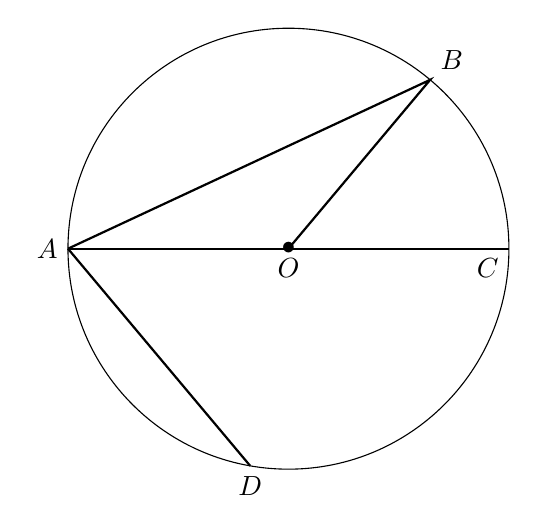
\begin{tikzpicture}[scale=0.7]
      \draw (0,0) circle[radius=4];
      \draw [thick]
      (-4,0) node[left] {$A$}--
      (0,0) node[below] {$O$}--
      (4,0) node[below left] {$C$};
      \draw [thick]
      (0,0) -- (50:4) node[above right] {$B$}--(-4,0);
      \draw [thick]
      (-4, 0)--
      (-100:4) node[below] {$D$};
      \node at (0,0) {$\bullet$};
    \end{tikzpicture}
    \end{multicols}

\newpage
\item Given circle $O$ with points on the circle $A$, $B$, $C$, $D$ as shown. Find each central angle measure.
  \begin{multicols}{2}
    \begin{enumerate} 
      \item $m\angle AOB =$
      \item $m\angle BOC =$
      \item $m\angle AOC =$
      \item What is the measure of the \emph{reflex angle} $m\angle AOC =$, i.e. the one containing point $D$ that is $>180^\circ$
      \end{enumerate}
      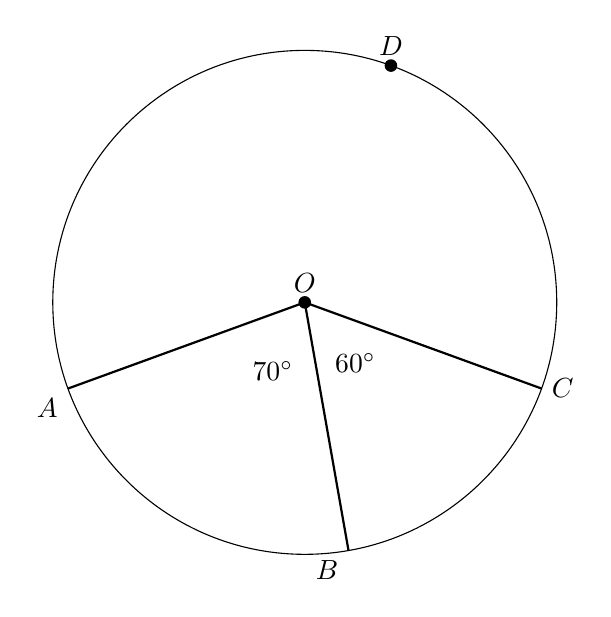
\begin{tikzpicture}[scale=0.8]
        \draw (0,0) circle[radius=4];
        \draw [thick]
        (-80:4) node[below left] {$B$}--
        (0,0) node[above] {$O$}--
        (-160:4) node[below left] {$A$};
        \draw [thick]
        (0,0) -- (-20:4) node[right] {$C$};
        %\node at (0,0) {$\bullet$};
        \fill (0,0) circle[radius=.1];
        \fill (70:4) circle[radius=.1]node[above]{$D$};
        \node at (-50:1.25) {$60^\circ$};
        \node at (-115:1.2) {$70^\circ$};
      \end{tikzpicture}
  \end{multicols}

\newpage
\item Lesson: A curved part of a circle is called an \emph{arc} and written $\wideparen{AB}$.
    \begin{multicols}{2}
    \raggedcolumns
    \begin{enumerate}[itemsep=0.5cm]
      \item Highlight arc $\wideparen{AB}$.
      \item An arc's degree measure equals its corresponding central angle measure. \\[0.25cm]
      If $m\angle AOB = 60^\circ$, what is the $m \wideparen{AB}$?
      \item A \emph{semicircle} is half of a circle.
      \item An arc smaller than half a circle is a \emph{minor} arc, one larger is a \emph{major} arc. \\[0.25cm]
      Which is a major arc, $\wideparen{AB}$ or $\wideparen{ACB}$?
    \end{enumerate}
    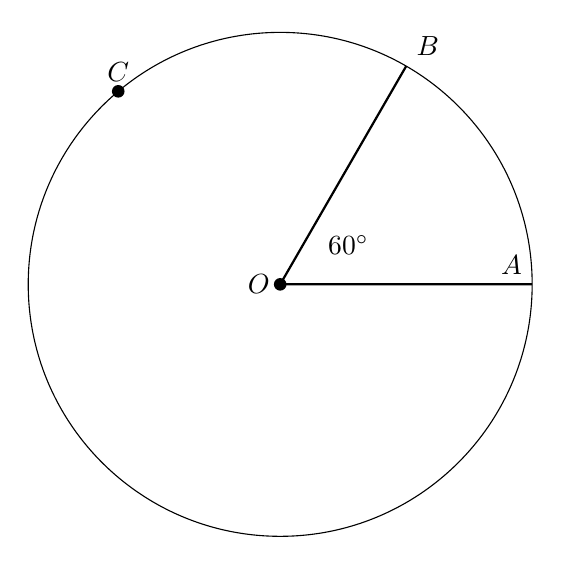
\begin{tikzpicture}[scale=0.8]
      \draw (0,0) circle[radius=4];
      \draw [thick]
      (0:4) node[above left] {$A$}--
      (0,0) node[left] {$O$}--
      (60:4) node[above right] {$B$};
      \fill (130:4) circle[radius=.1]node[above]{$C$};
      \fill (0,0) circle[radius=.1];
      \node at (30:1.25) {$60^\circ$};
    \end{tikzpicture}
    \end{multicols}

\newpage
\item A regular hexagon is inscribed in a circle with a radius $r=12$, as shown.
    \begin{multicols}{2}
    \raggedcolumns
    \begin{enumerate}[itemsep=2cm]
      \item Find the circumference of the circle in terms of $\pi$. ($C=2\pi r$)
      \item How long is the curved part of the circle from point $A$ to $B$, $\wideparen{AB}$?
      \item What is the degree measure of the arc from point $A$ to $C$,  $m \wideparen{AC}$?
    \end{enumerate}
    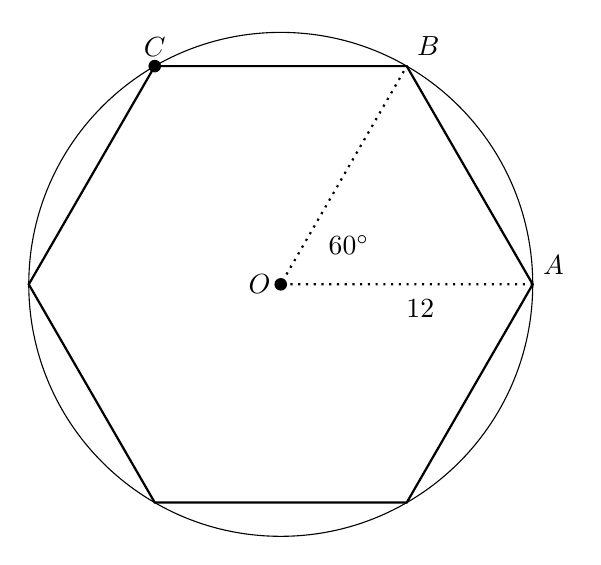
\begin{tikzpicture}[scale=0.8]
      \draw (0,0) circle[radius=4];
      \draw [thick, dotted]
      (0:4) node[above right] {$A$}--
      (0,0) node[left] {$O$}--
      (60:4) node[above right] {$B$};
      \draw [thick]
      (0:4) -- (60:4)-- (120:4)-- (180:4)-- (240:4)-- (300:4)-- cycle;
      \fill (120:4) circle[radius=.1]node[above]{$C$};
      \fill (0,0) circle[radius=.1];
      \node at (30:1.25) {$60^\circ$};
      \node at (-10:2.25) {$12$};
    \end{tikzpicture}
    \end{multicols}
    
\newpage
\item What is an equation of circle O shown in the graph below?
  \begin{center}
    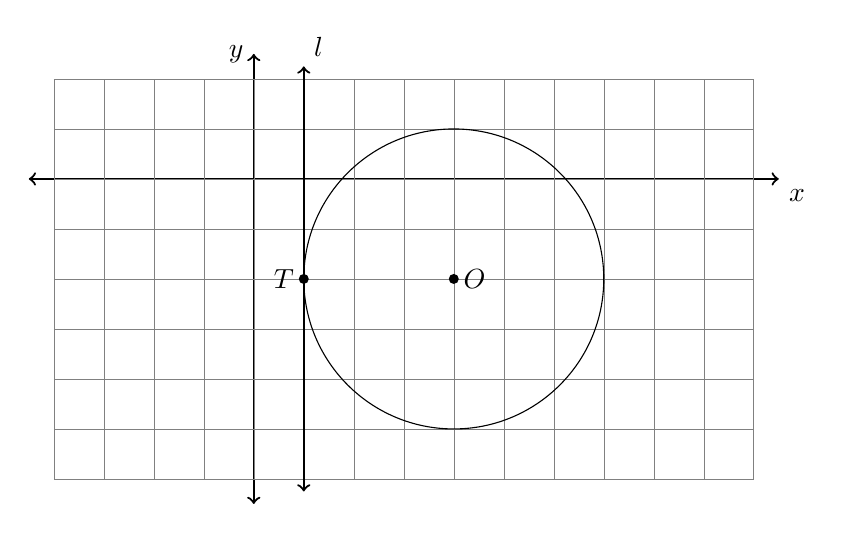
\begin{tikzpicture}[scale=.635]
      \draw [thick, <->] (-4.5,0) -- (10.5,0) node [below right] {$x$};
      \draw [thick, <->] (0,-6.5)--(0,2.5) node [left] {$y$};
      \draw [help lines] (-4,-6) grid (10,2);
      \draw (4,-2) circle[radius=3];
      \fill (4,-2) circle[radius=.1]node[right]{$O$};
      \draw [thick, <->] (1,-6.25) -- (1,2.25) node [above right] {$l$};
      \fill (1,-2) circle[radius=.1]node[left]{$T$};
    \end{tikzpicture}
  \end{center}
  \begin{multicols}{2}
    \begin{enumerate}
      \item $(x-4)^2+(y+2)^2=9$
      \item $(x-4)^2+(y+2)^2=9^2$
      \item $(x+2)^2+(y-4)^2=9$
      \item $(x+2)^2+(y-4)^2=9^2$
    \end{enumerate}
  \end{multicols}
  Write down the coordinates of the point of tangency $T$ and the equation of the tangent line $l$.
     
\newpage
\item What are the coordinates of the center and the length of the radius of the circle whose equation is $(x-4)^2+(y+3)^2=16$?
    \begin{enumerate}
      \item center $(-4,3)$ and radius 8
      \item center $(4,-3)$ and radius 4
      \item center $(-4,3)$ and radius 4
      \item center $(4,-3)$ and radius 8
    \end{enumerate}

\newpage
\item What is the equation of a circle with center $(5,0)$ and radius $r=5$?\\[0.5cm]
  Graph the circle in Graspable Math or Geogebra and paste the image here.

\newpage
\item Given the diameter of circle $C$ is $\overline{AB}$, $A(3,2)$ and $B(9,10)$, find the length of $\overline{AB}$ and hence, the radius of the circle.\\[0.25cm]
Find the equation of the circle. Graph the circle and its diameter.


\end{enumerate}
\end{document}